\documentclass[xelatex,mathserif,serif]{beamer}
\usetheme{PaloAlto}
\usecolortheme{beaver}

% increased bullet spacing
\newlength{\wideitemsep}
\setlength{\wideitemsep}{\itemsep}
\addtolength{\wideitemsep}{3pt}
\let\olditem\item
\renewcommand{\item}{\setlength{\itemsep}{\wideitemsep}\olditem}

% xelatex
\usepackage{fontspec}
\usepackage{xunicode}
\usepackage{xltxtra}

\usepackage{amsmath}
\usepackage{amssymb}
\usepackage{enumerate}

\usepackage{graphicx}
\DeclareGraphicsExtensions{.png,.eps,.jpg}

% languages
\usepackage{fixlatvian}
\usepackage{polyglossia}
\setdefaultlanguage{latvian}
\setotherlanguages{english,russian}

\author{Emīls Šolmanis}
\title{GPS datu segmentēšana}
\date{\today}

\begin{document}

\frame{\titlepage}

\begin{frame}
  \frametitle{Kas ir GPS?}
  \begin{itemize}
  \item Globālā pozicionēšanas sistēma
  \item Ar vairāku satelītu palīdzību nosaka uztvērēja atrašanās vietu
  \item Mūsdienās precizitāte (civilajām) ierīcēm ~ 5 - 10 metri
  \end{itemize}
\end{frame}

\begin{frame}
  \frametitle{Cik izplatīts ir GPS?}
  \begin{itemize}
  \item Jebkurā mūsdienīgā mobilajā tālrunī
  \item Bieži iespēja pievienot auto komplektācijai
  \item Ļoti daudz viedtelefonu lietotņu, kas popularizē GPS datu lietošanu:
    \begin{itemize}
    \item Endomondo
    \item FourSquare, u.c.
    \end{itemize}
  \item ASV FKK lēmuma rezultātā paredzams, ka popularitāte tikai turpinās augt
  \end{itemize}
\end{frame}

\begin{frame}
  \frametitle{Kādi dati tiek lietoti darbā?}
  \begin{itemize}
  \item Ierakstīti ar \emph{Samsung Galaxy Note GT-N7000} viedtālruni
  \item Trijnieki \emph{(garums, platums, laiks)}
  \item Iztveršanas intervāls 1 sekunde
  \end{itemize}
\end{frame}

\begin{frame}
  \frametitle{Kādi dati ir ierakstīti?}
  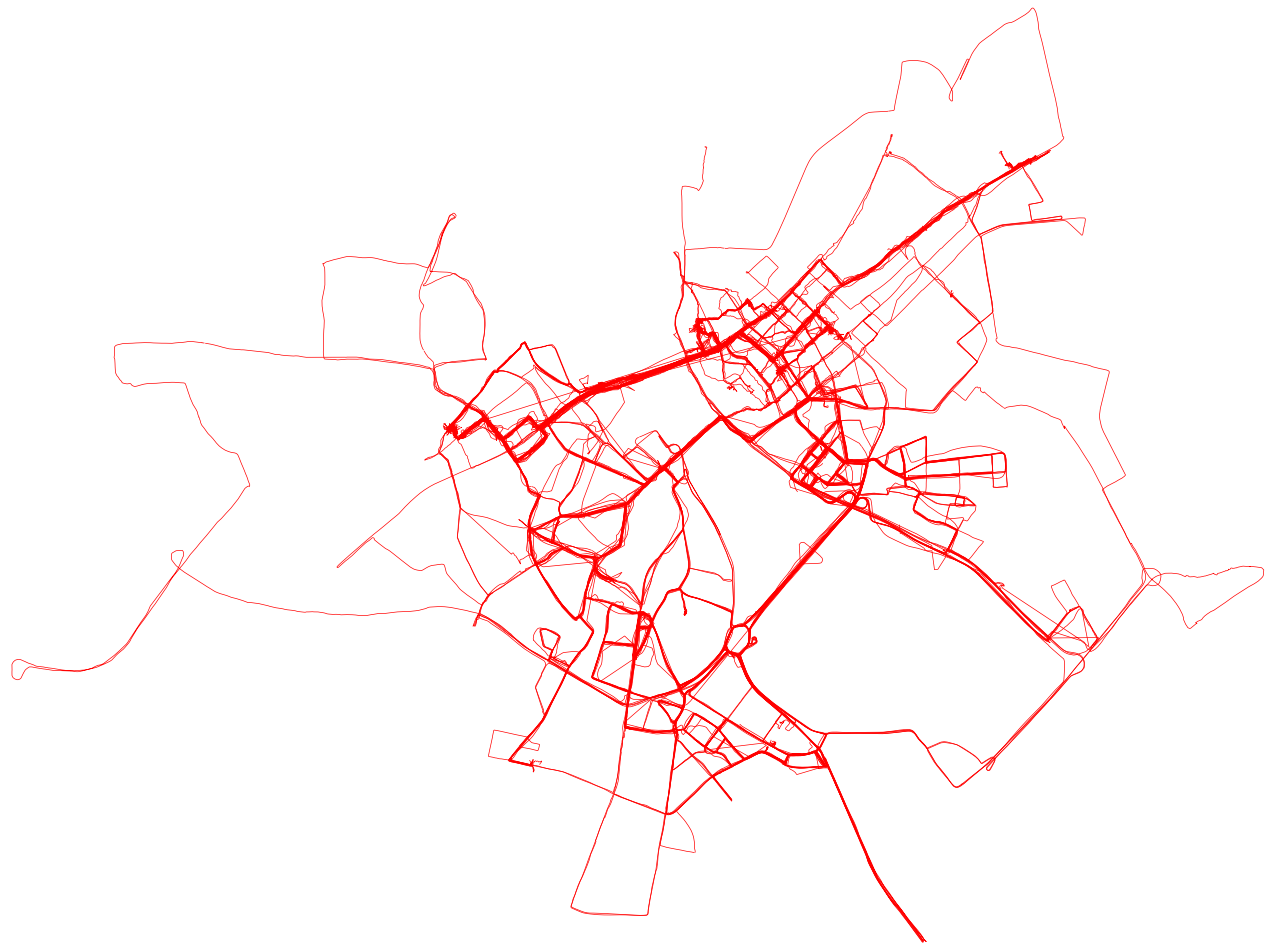
\includegraphics[scale=0.3]{img/all_trails}
\end{frame}

\begin{frame}
  \frametitle{Kāds ir darba mērķis?}
  \begin{itemize}
  \item Sadalīt datus segmentos pa transporta veidiem
  \item Sagrupēt iegūtos segmentus pēc vienādiem transporta veidiem
  \end{itemize}
\end{frame}

\begin{frame}
  \frametitle{Kas ir klasterizācija?}
  \begin{itemize}
    \item \textbf{Mašīnmācīšanās} ir mākslīgā intelekta apakšnozare, kas veido uzvedības modeļus 
      balstoties uz empīriskiem datiem
    \item \textbf{Klasterizācija} ir mašīnmācīšanās metode, kas grupē datu paraugus pēc kādas
      kopīgas pazīmes
  \end{itemize}
\end{frame}

\begin{frame}
  \frametitle{Kāpēc segmentēt GPS datus?}
  \begin{itemize}
    \item Lai kādam nebūtu dati jāiezīmē manuāli
    \item Personalizētas ceļu plānošanas sistēmas
    \item Pilsētas infrastruktūras optimizācija
  \end{itemize}
\end{frame}

\begin{frame}
  \frametitle{Kādi ir esošie risinājumi?}
  \emph{GeoLife}
  \begin{itemize}
    \item \emph{Microsoft Research Asia} projekts
    \item Izmanto lēmumu kokus, lai klasificētu segmentus
    \item Attiecīgi atpazīstamo transporta veidu skaits – ierobežots un autoru noteikts
  \end{itemize}
\end{frame}

\begin{frame}
  \frametitle{Kāpēc neuzraudzītā mašīnmācīšanās?}
  \begin{itemize}
  \item Nepalaiž garām jaunus, iepriekš neredzētus transporta veidus
  \item Algoritms noturīgāks pret nevienmērīgi sadalītām klasēm
  \end{itemize}
\end{frame}

\begin{frame}
  \frametitle{Kādas ir iespējamās pazīmes?}
  \begin{itemize}
    \item Nav pārāk daudz, jo maz pieejamās informācijas
    \item Pamatā jebkas ko var izgūt no attāluma / laika / virziena kombinācijas, piemēram
      \begin{itemize}
      \item Ātrums
      \item Paātrinājums
      \item Virzienu maiņas
      \end{itemize}
  \end{itemize}
\end{frame}

\begin{frame}
  \frametitle{Ātrums}
  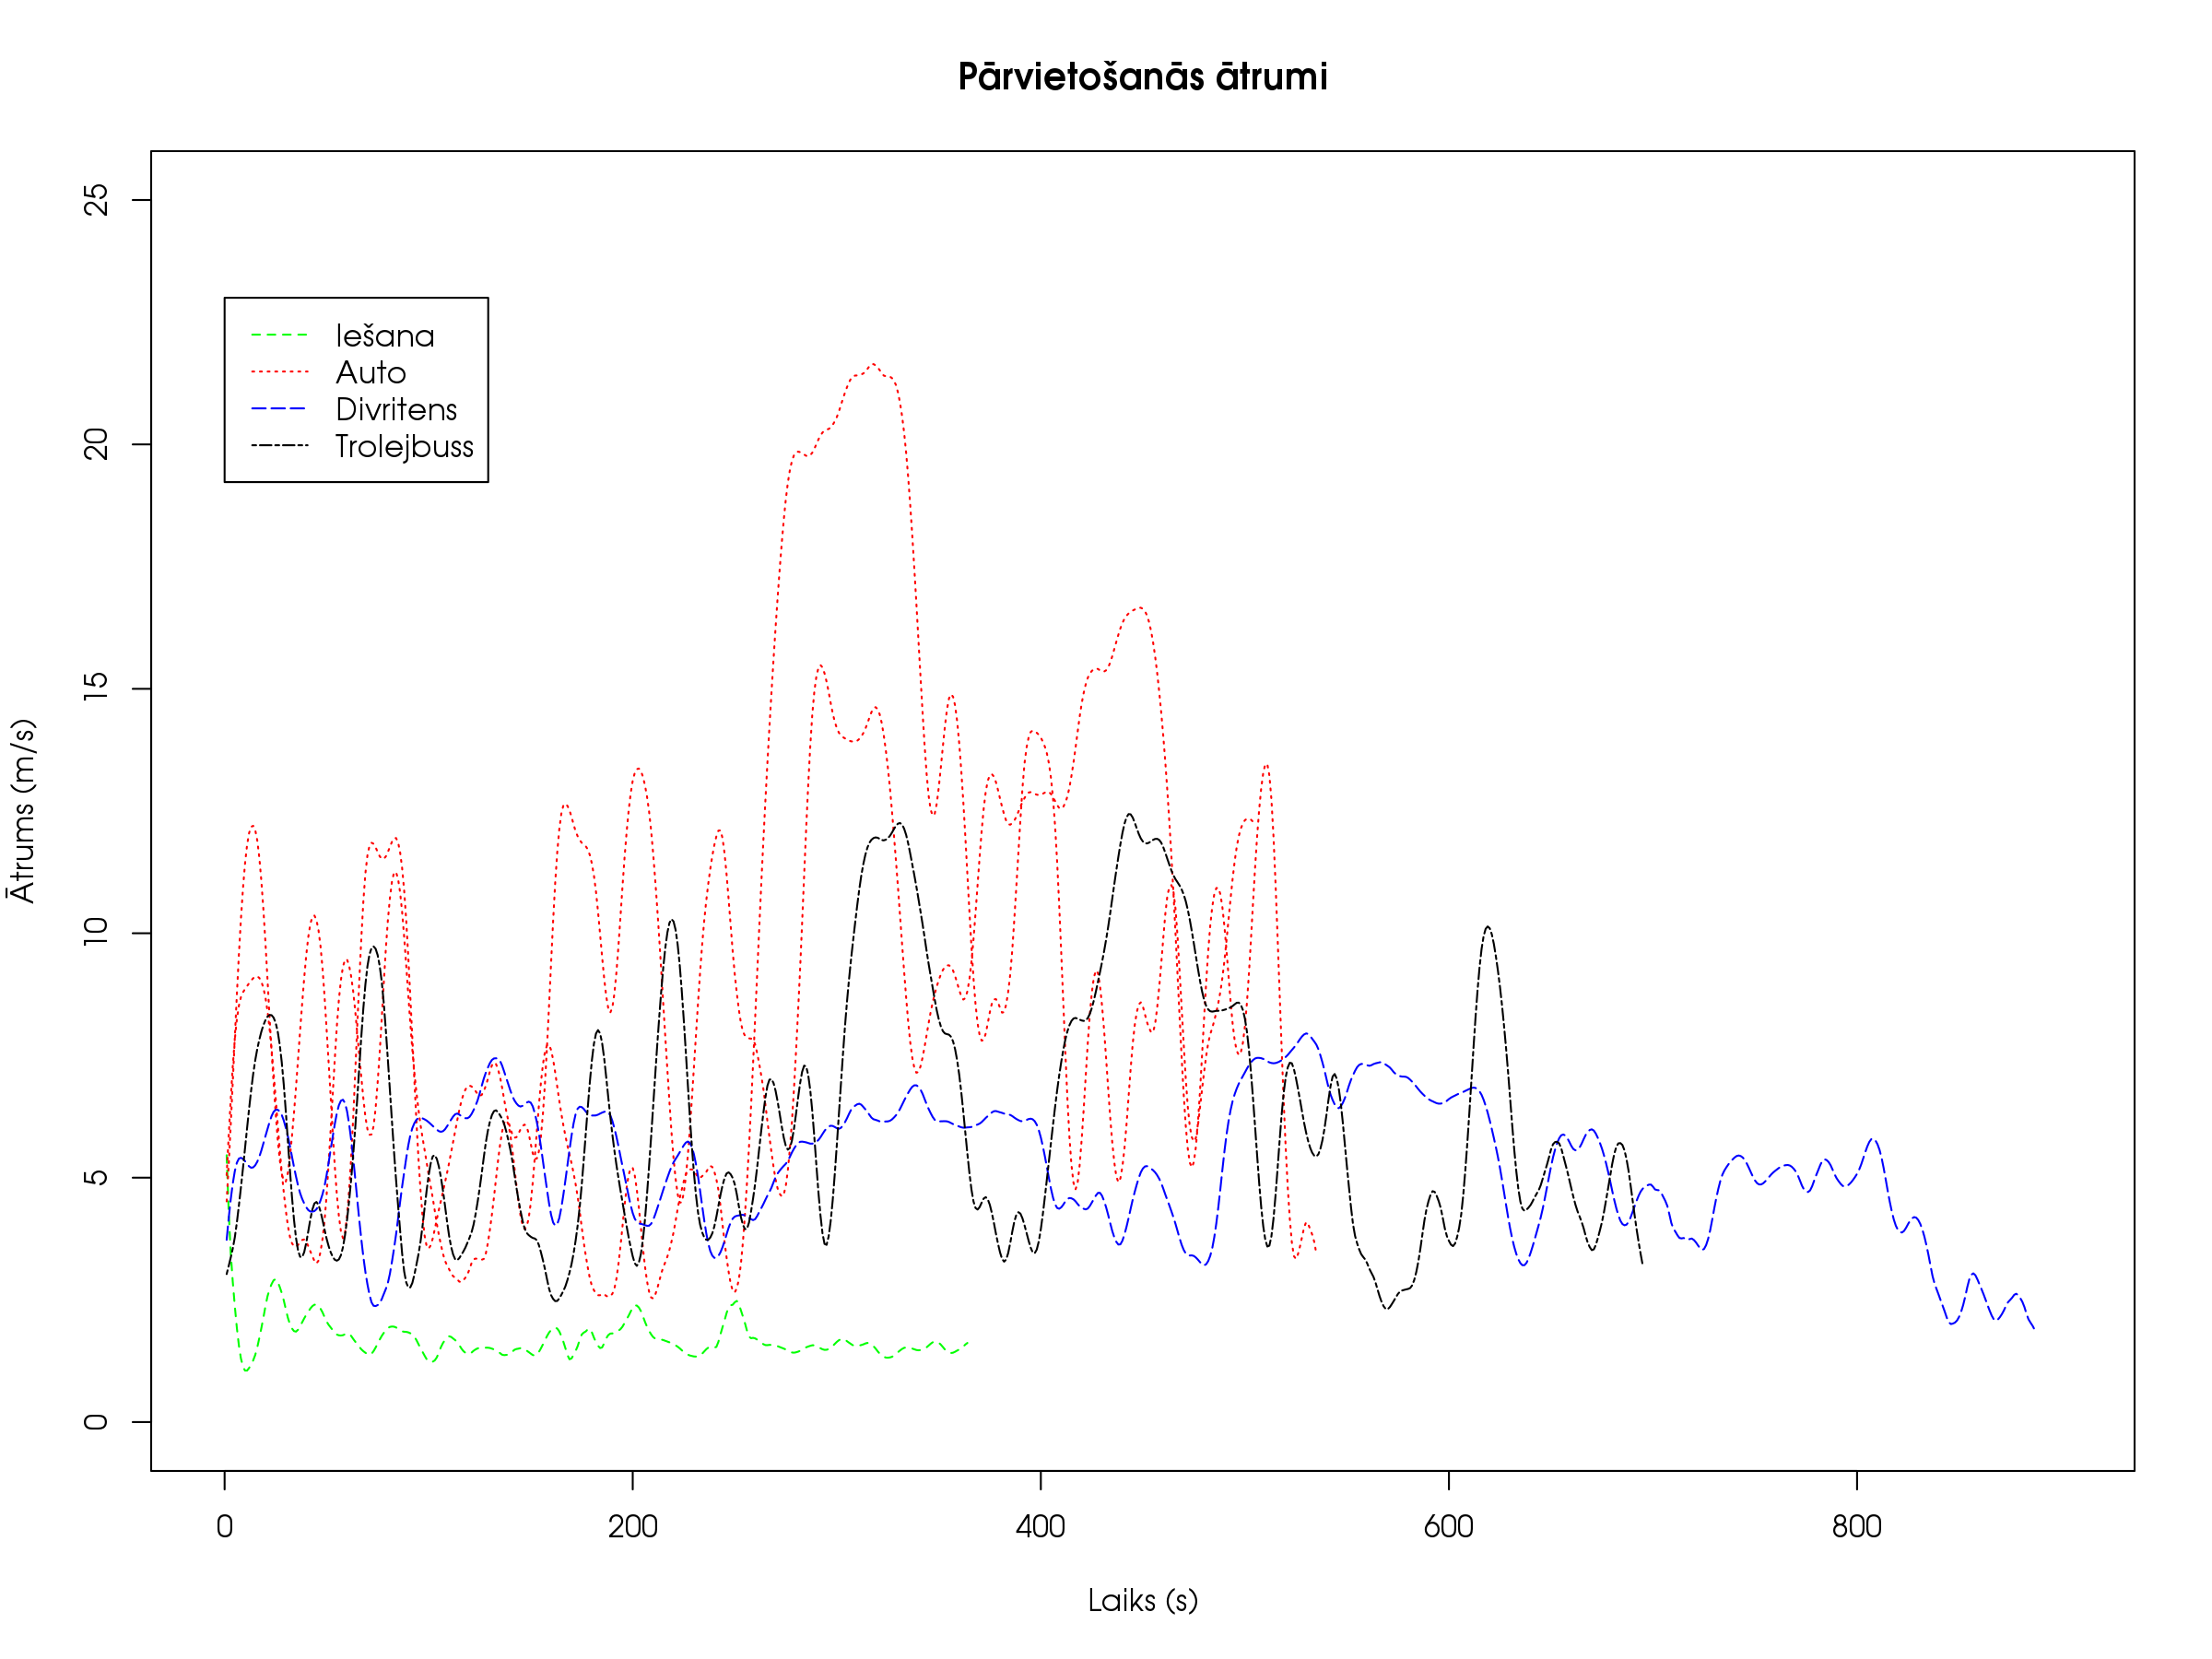
\includegraphics[scale=0.3]{img/speed_comparison}
\end{frame}

\begin{frame}
  \frametitle{Paātrinājums}
  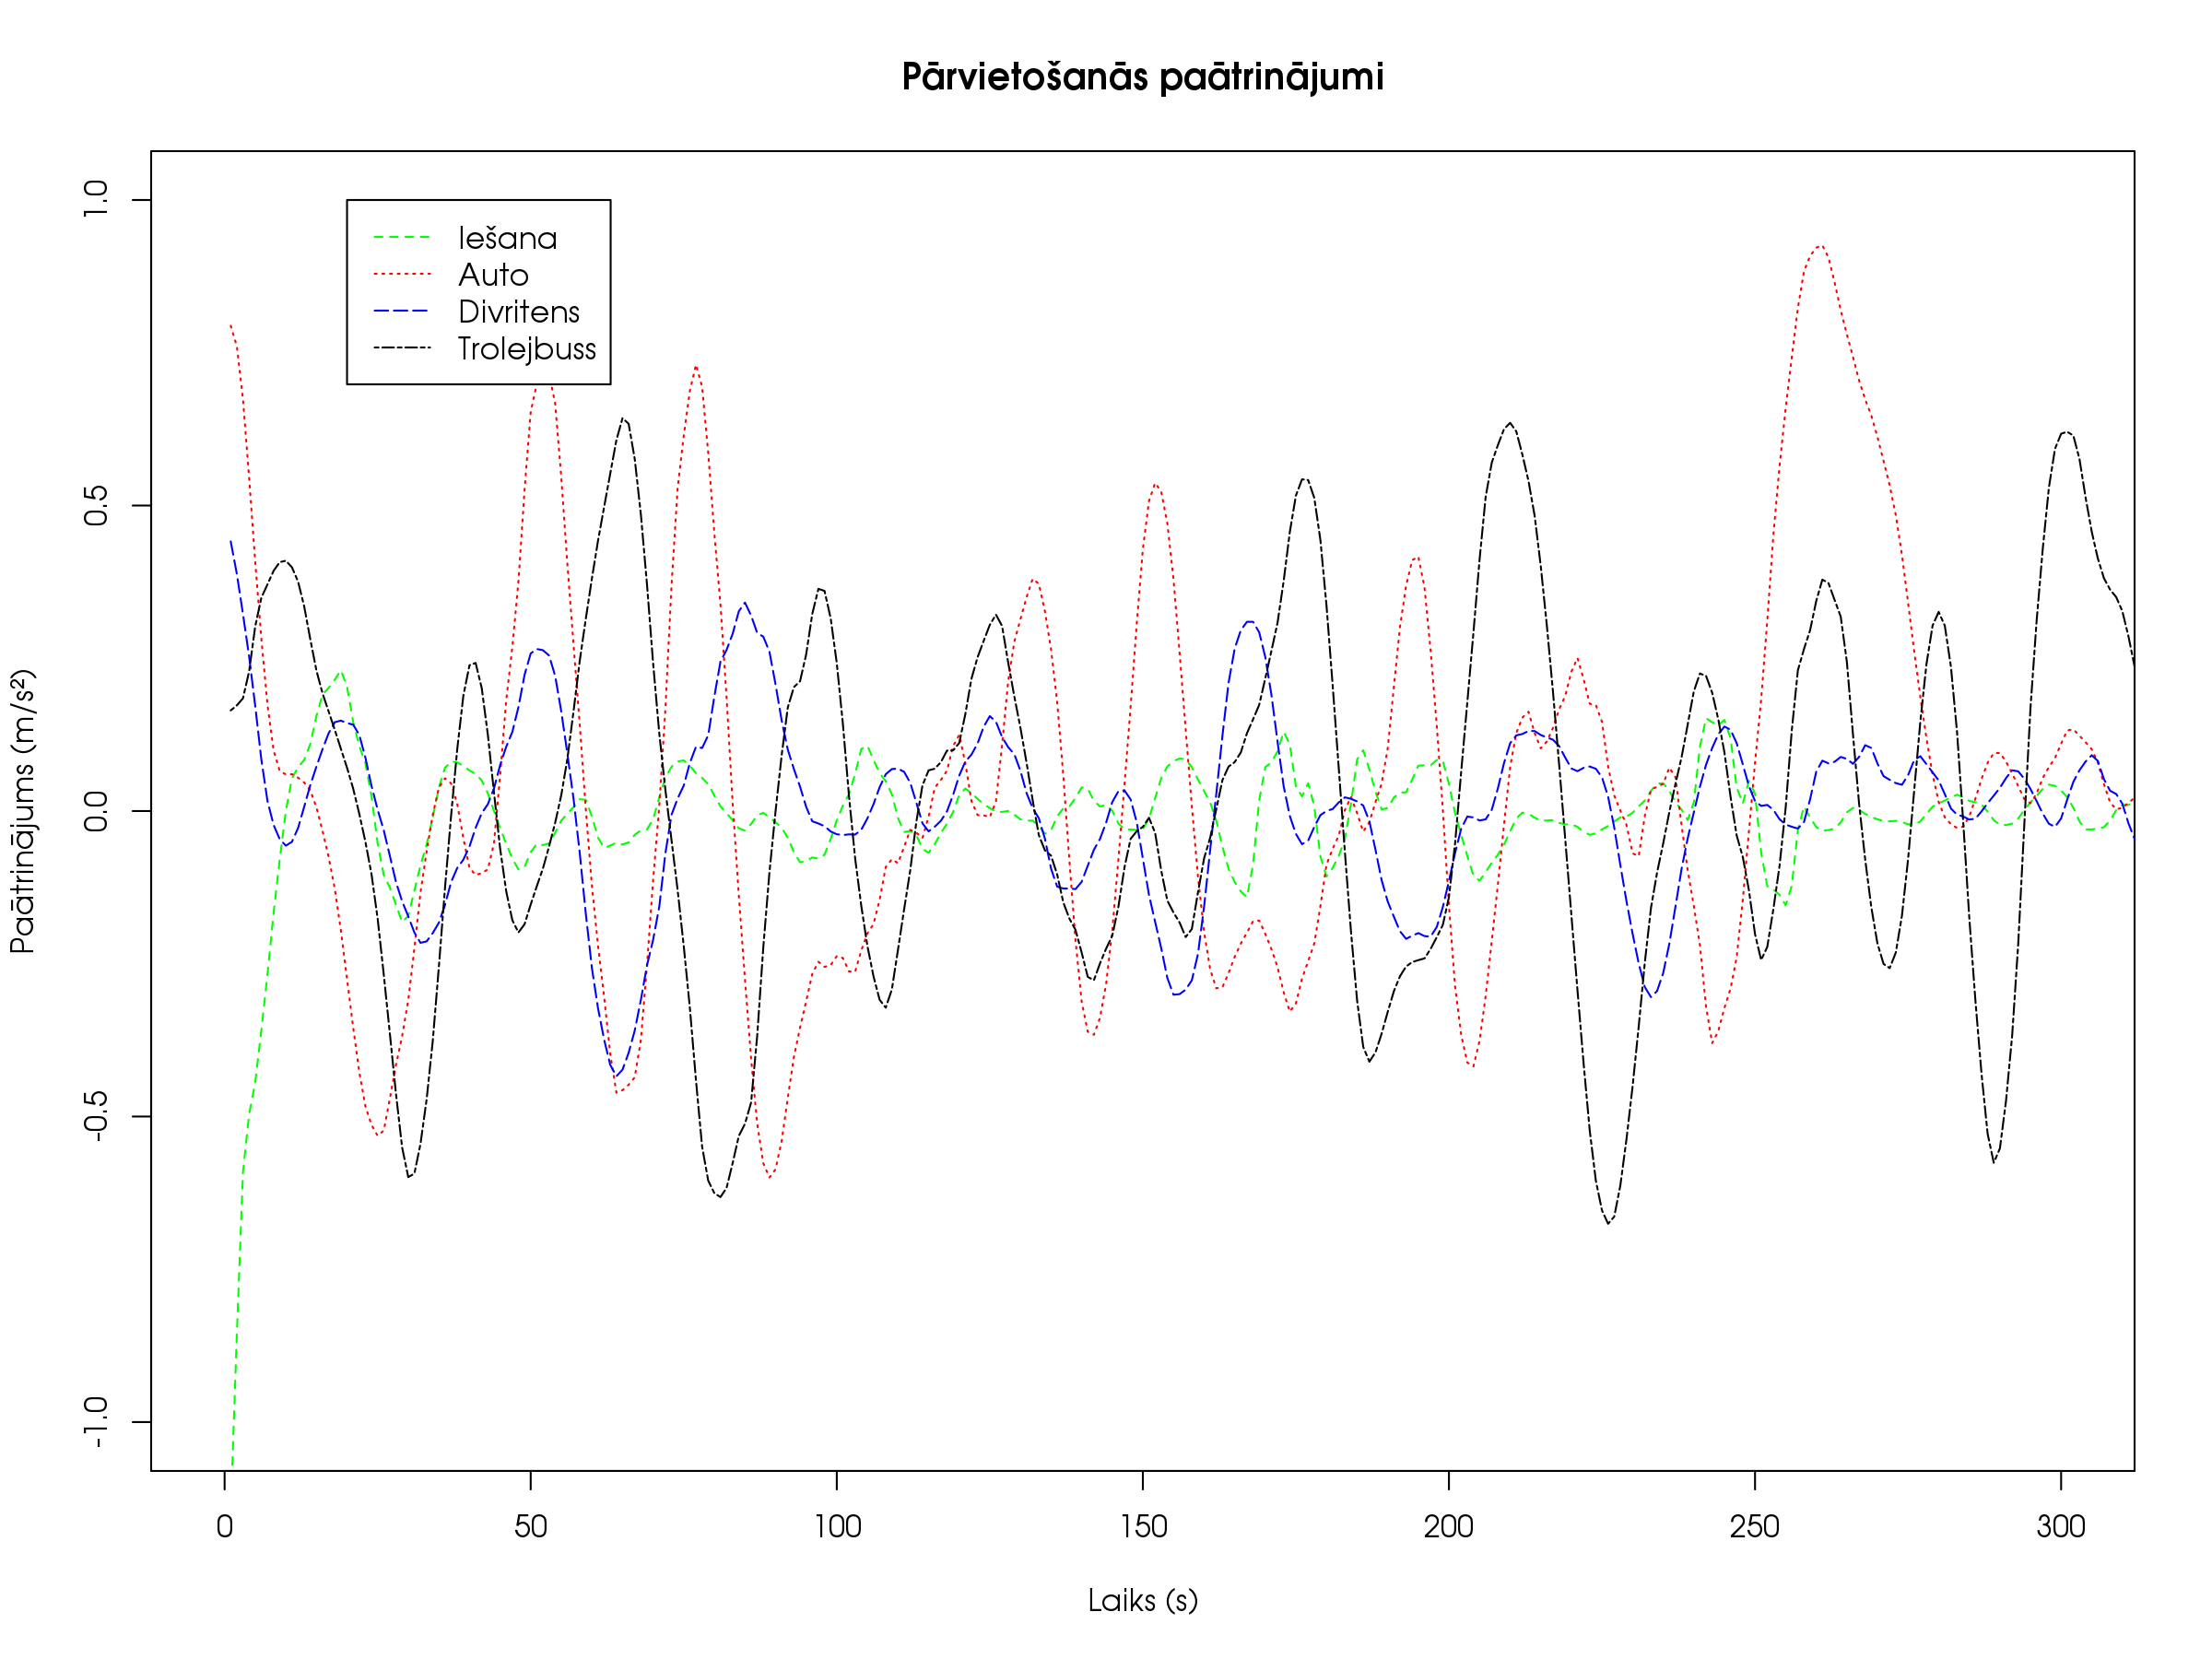
\includegraphics[scale=0.3]{img/acceleration_comparison}
\end{frame}

\begin{frame}
  \frametitle{Paātrinājuma spektrālā analīze}
  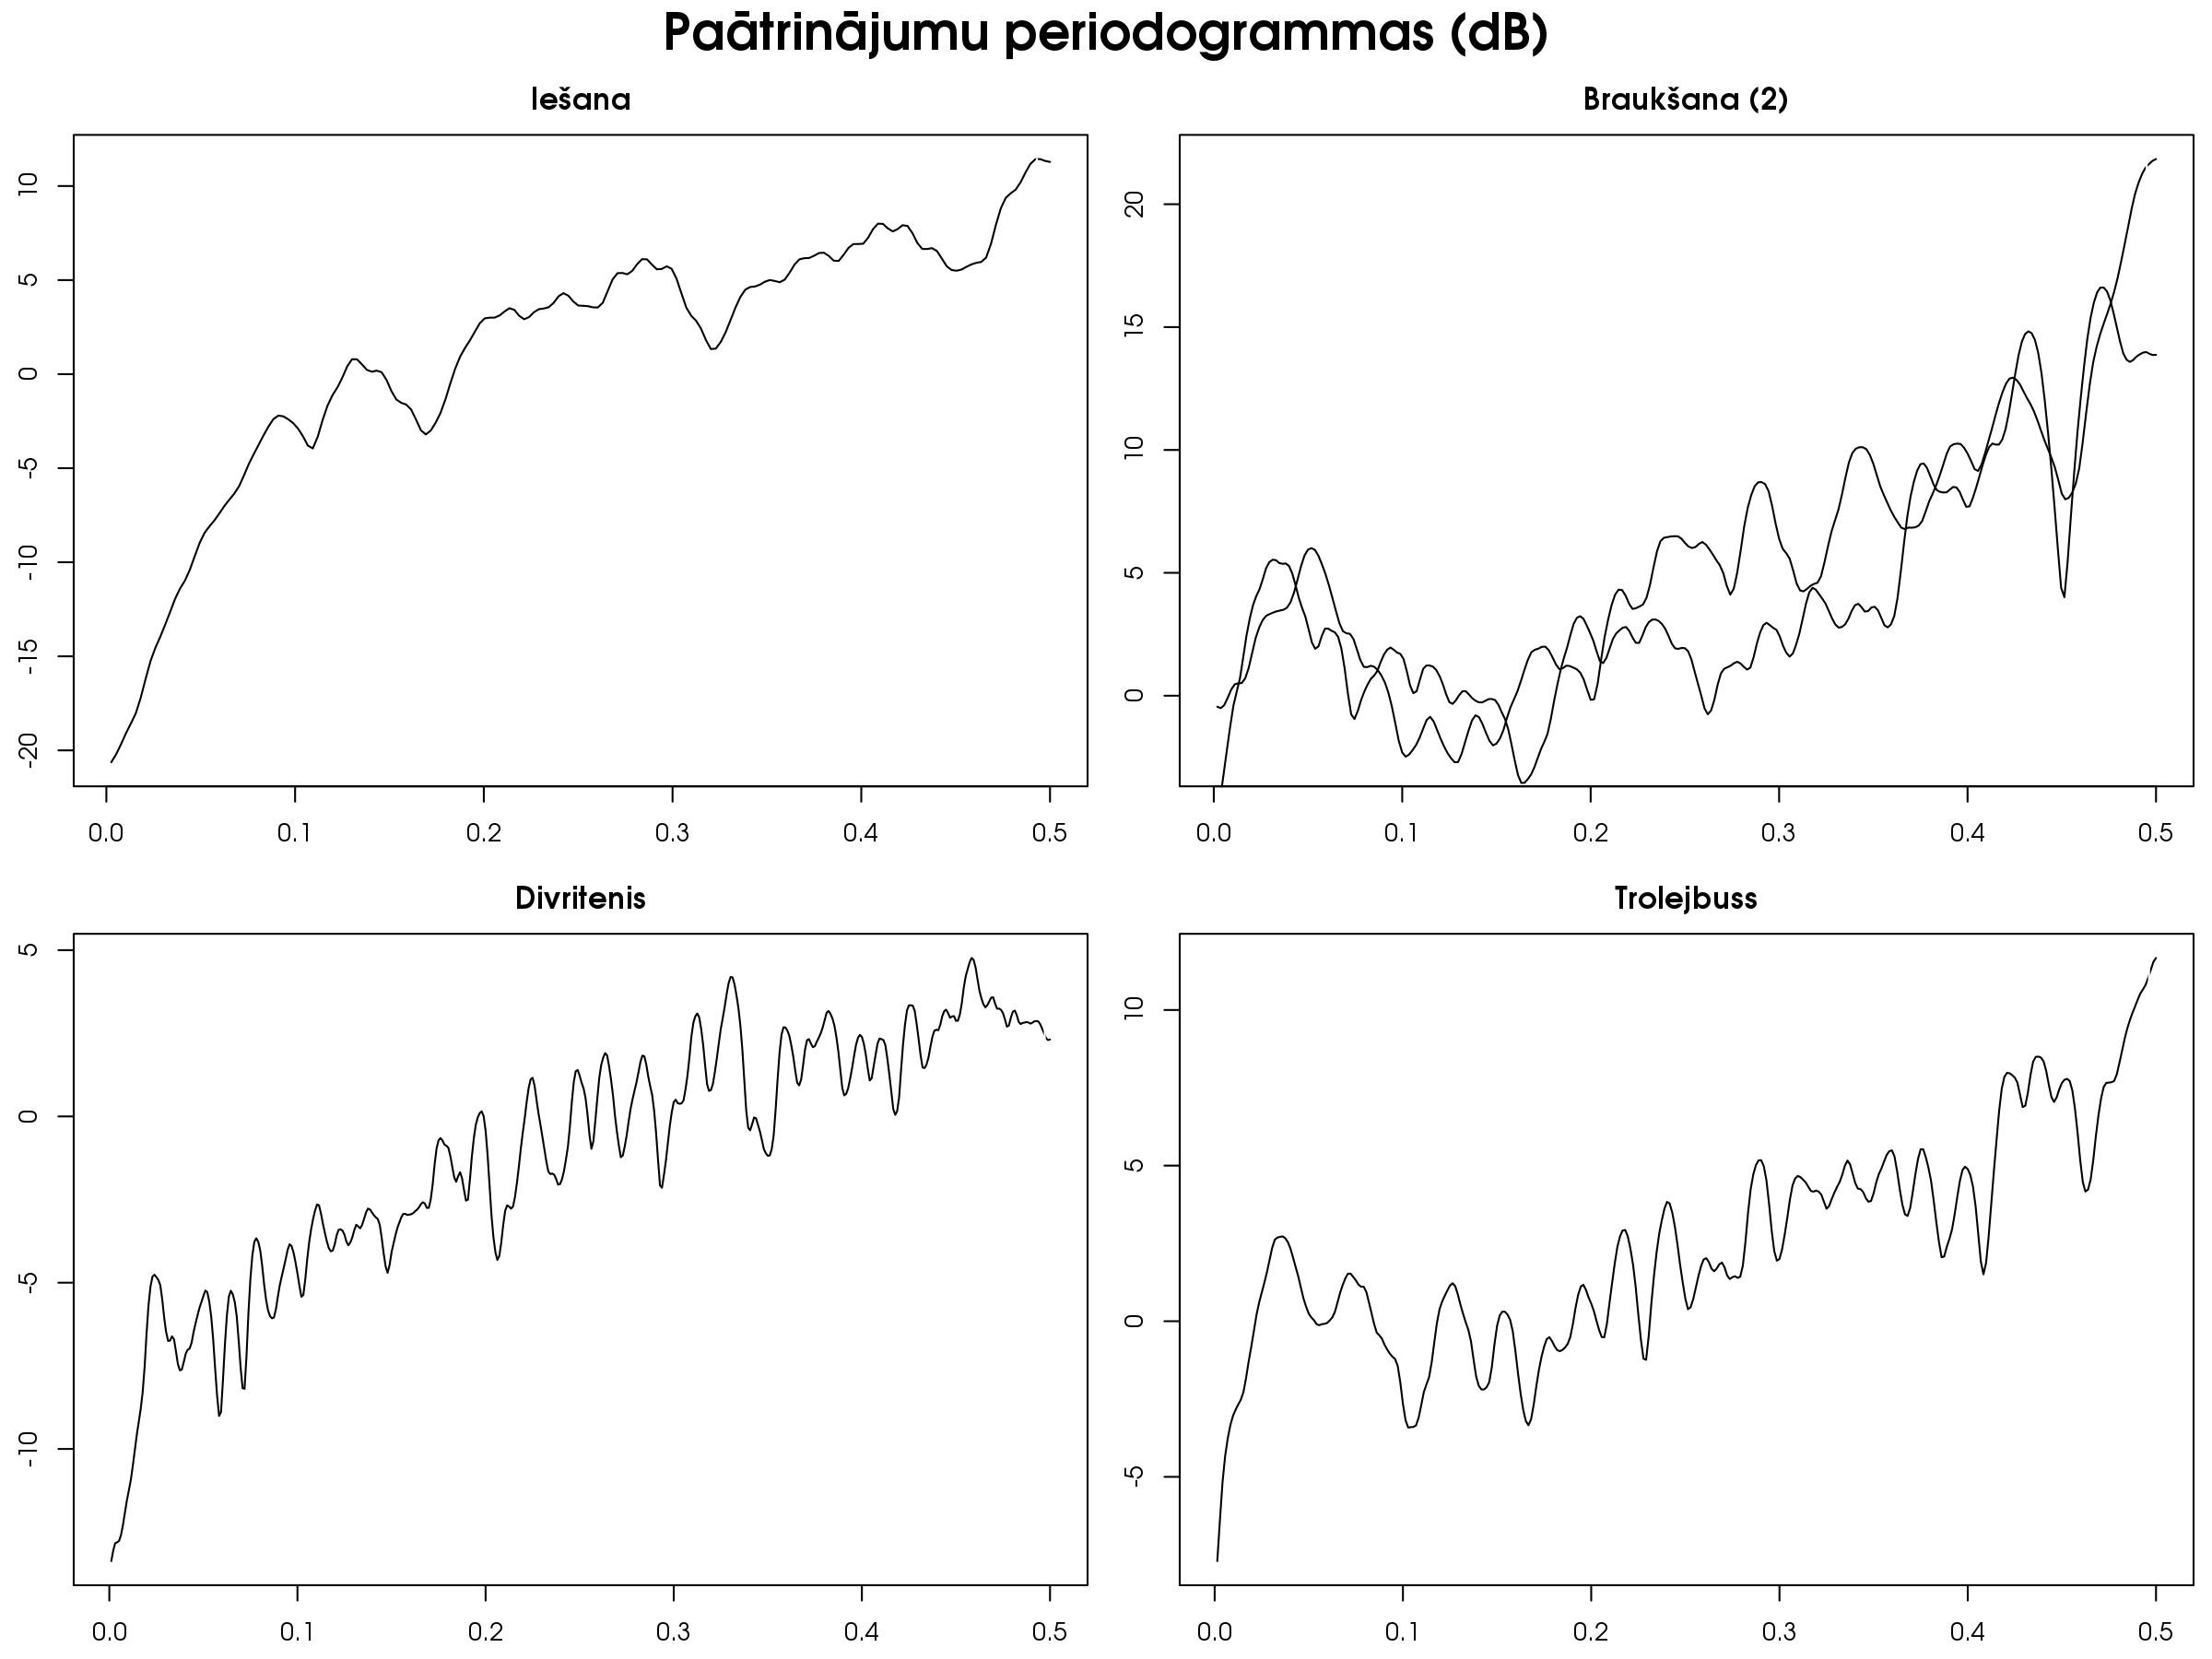
\includegraphics[scale=0.3]{img/periodograms}
\end{frame}

\begin{frame}
  \frametitle{Kādi ir klasterizācijas rezultāti?}
  \begin{itemize}
    \item Viduvēji – liela daļa datu pareizi sagrupēti, bet ir manāmas kļūdas
    \item Bet atrasto klasteru skaits un sadalījums apmēram atbilst datu kopā esošajam
  \end{itemize}
\end{frame}

\begin{frame}
  \frametitle{Cik klasteri?}
  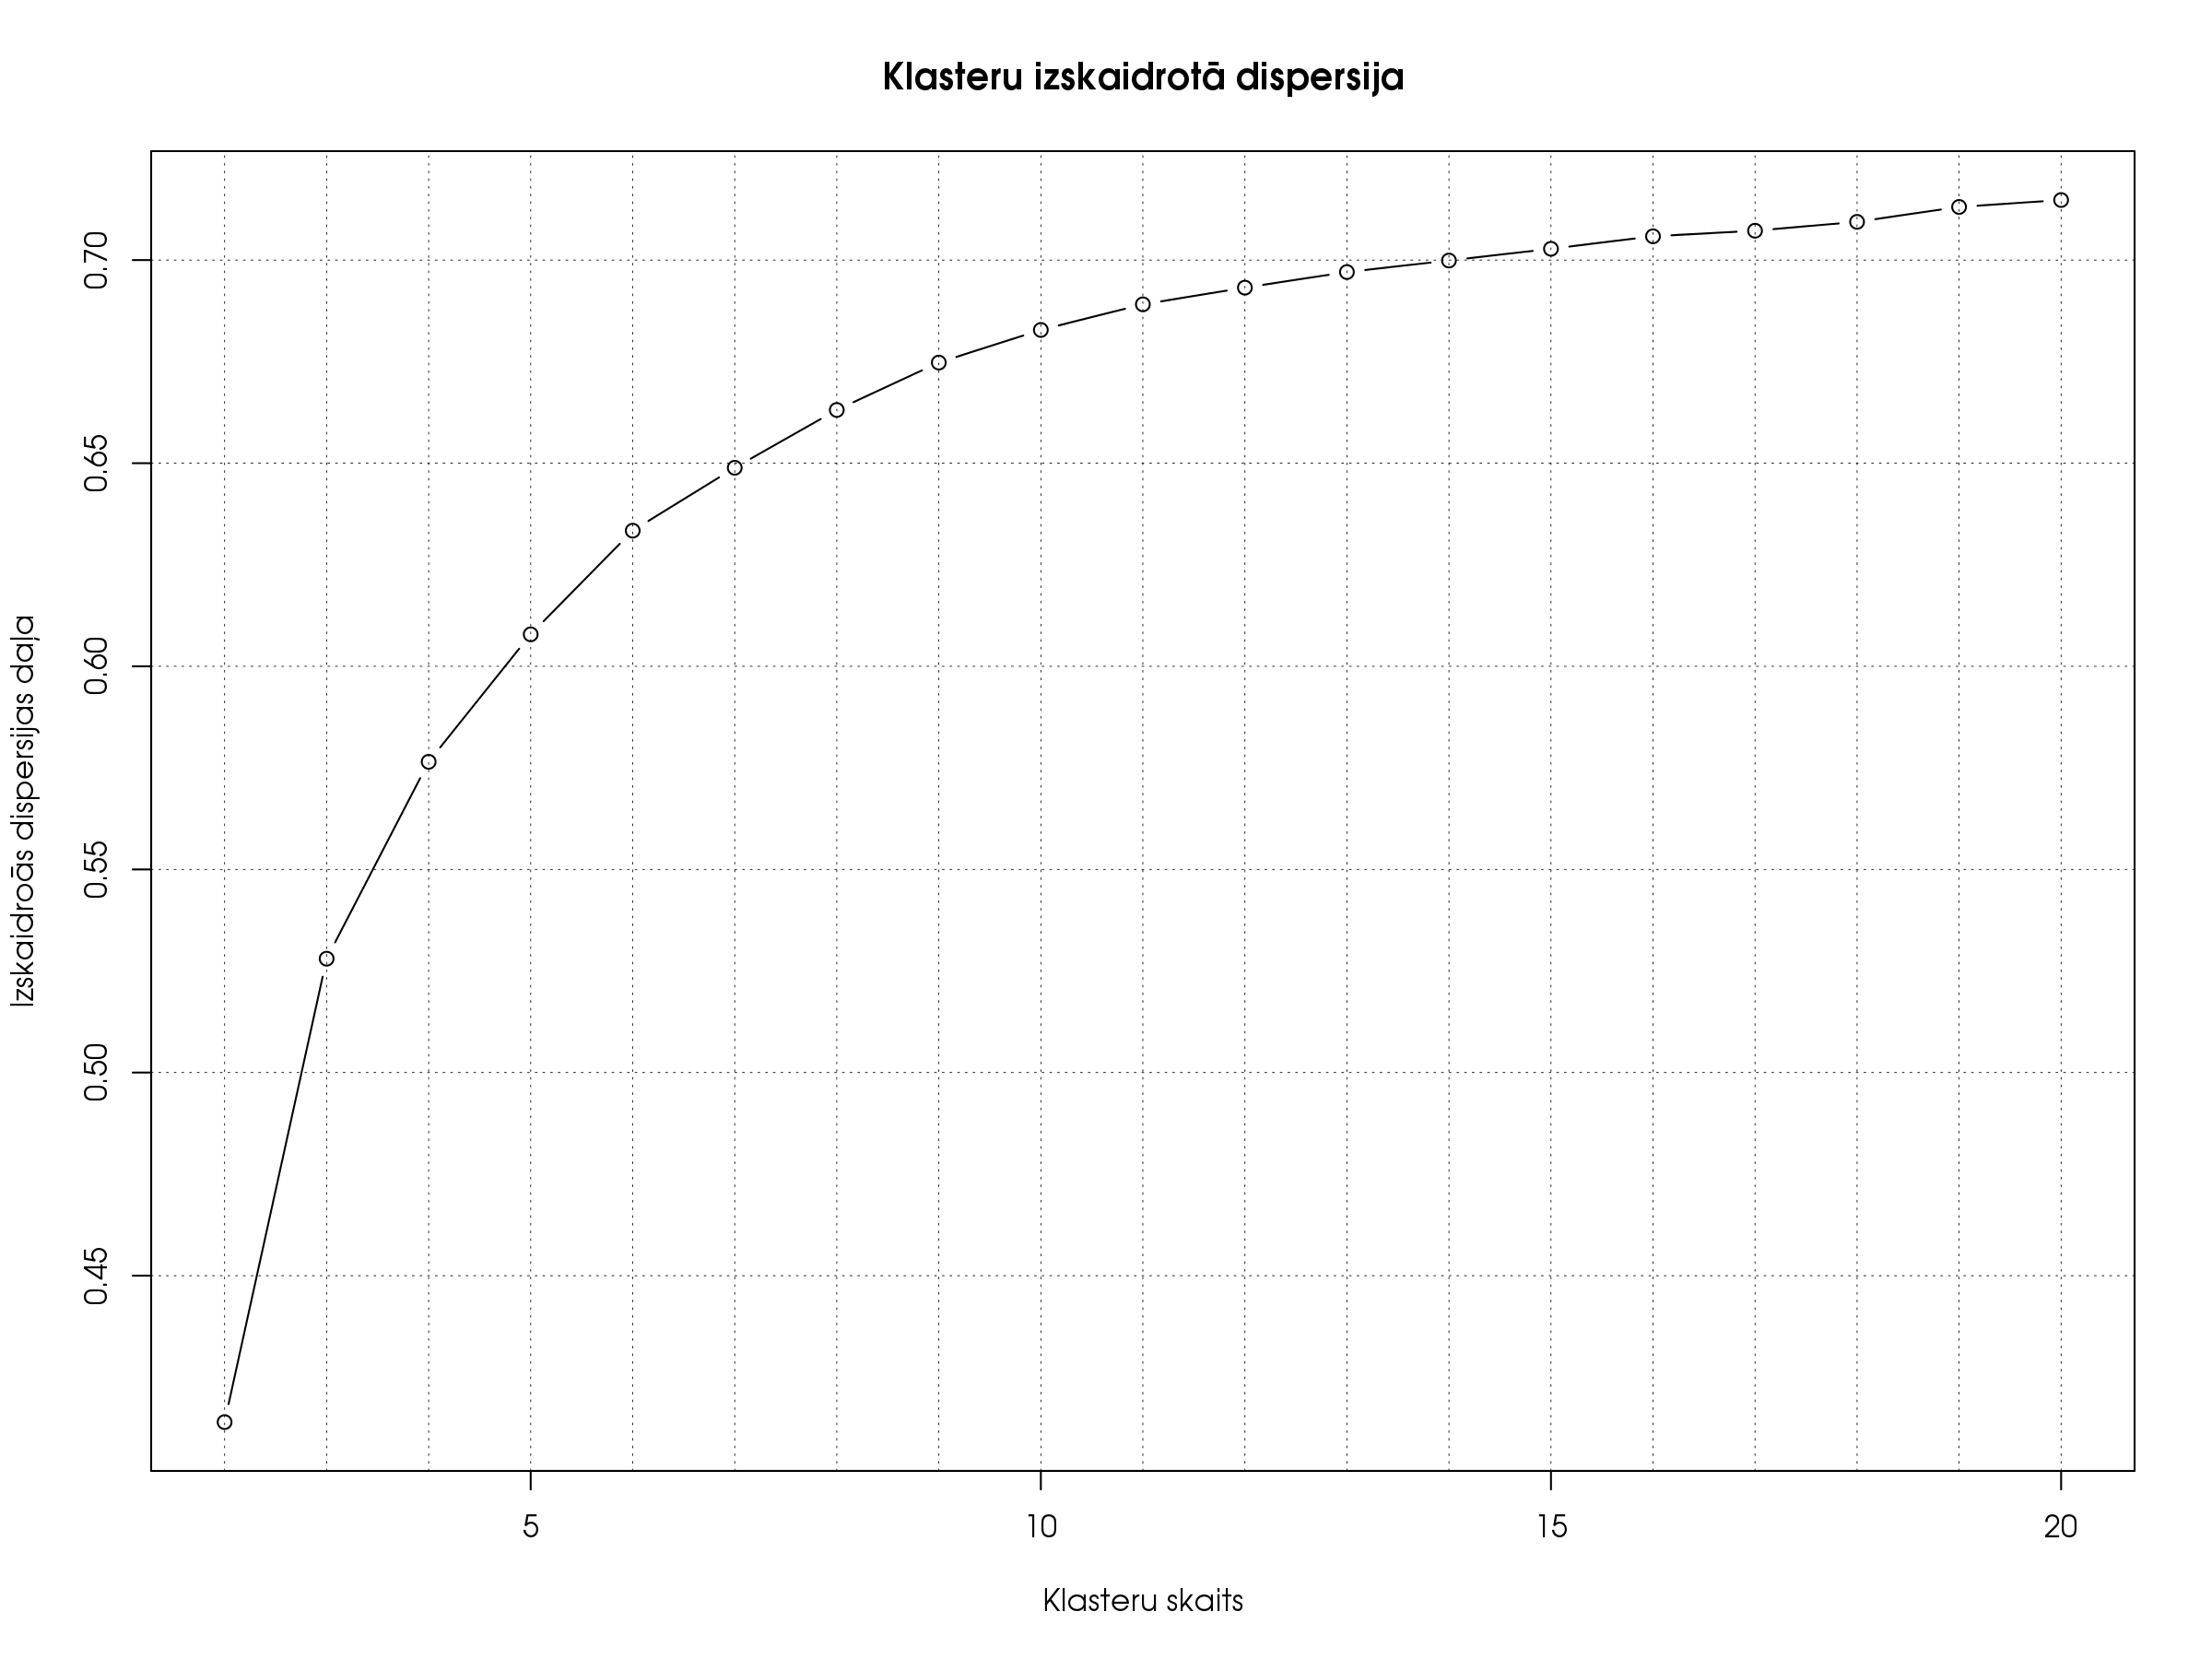
\includegraphics[scale=0.3]{img/kmeans_elbow}
\end{frame}

\begin{frame}
  \frametitle{Kā tas izskatās?}
  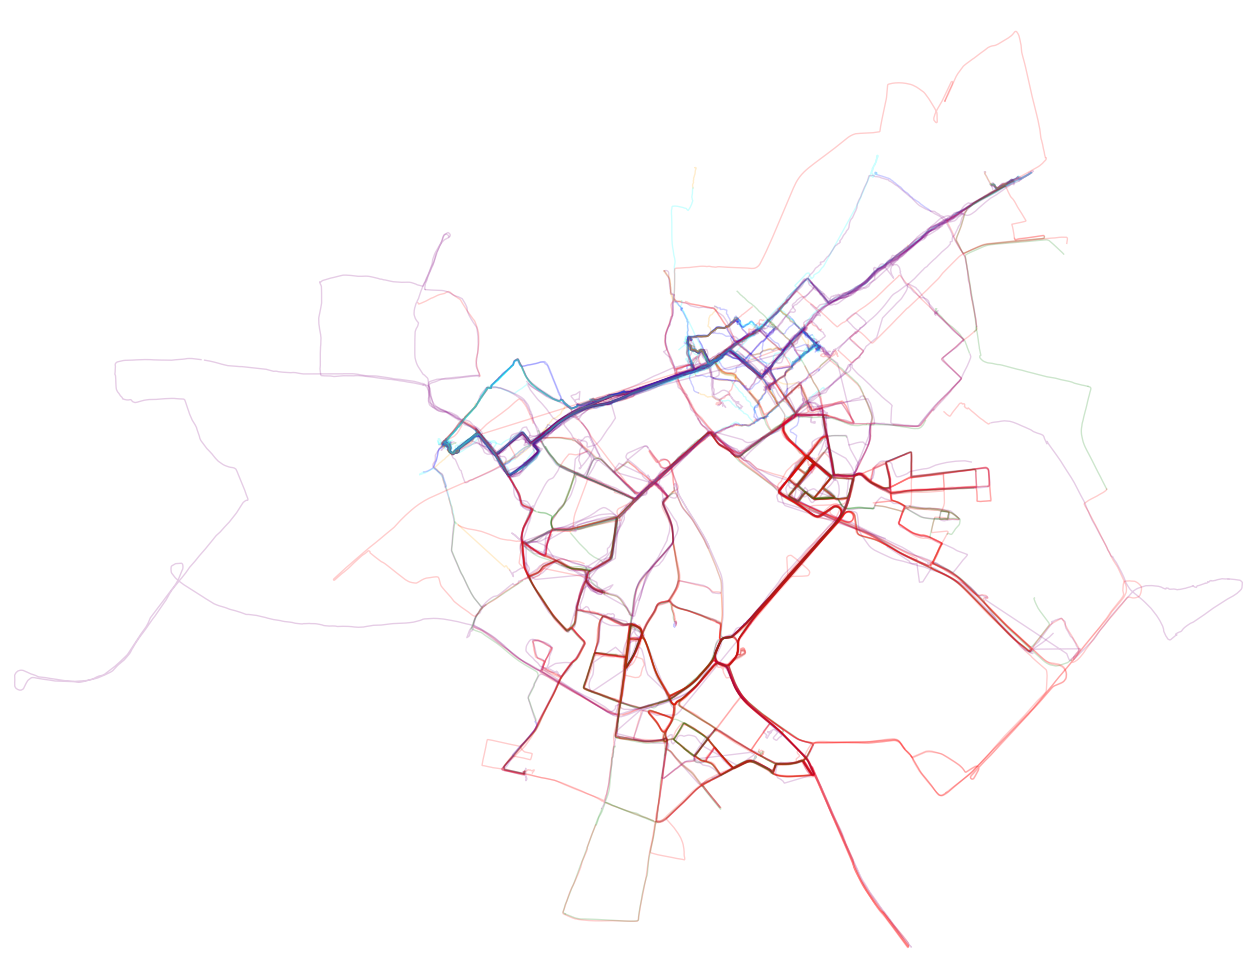
\includegraphics[scale=0.3]{img/clustered_trails}
\end{frame}

\begin{frame}
  \frametitle{Kādas ir kļūdas?}
  \begin{itemize}
  \item Gan pirmajā, gan otrajā algoritma posmā
  \item Vairāki posmi nepareizi klasificēti
  \item Ir segmenti, kas tiek konsekventi nepareizi iedalīti kā staigāšanas segmenti
  \item Pirmajā posmā mēdz būt "trokšņi", kuru rezultātā tiek nepareizi nošķelts mazs segments 
    pa vidu lielākam
  \end{itemize}
\end{frame}

\begin{frame}
  \frametitle{Nepareizi nošķelts segments}
  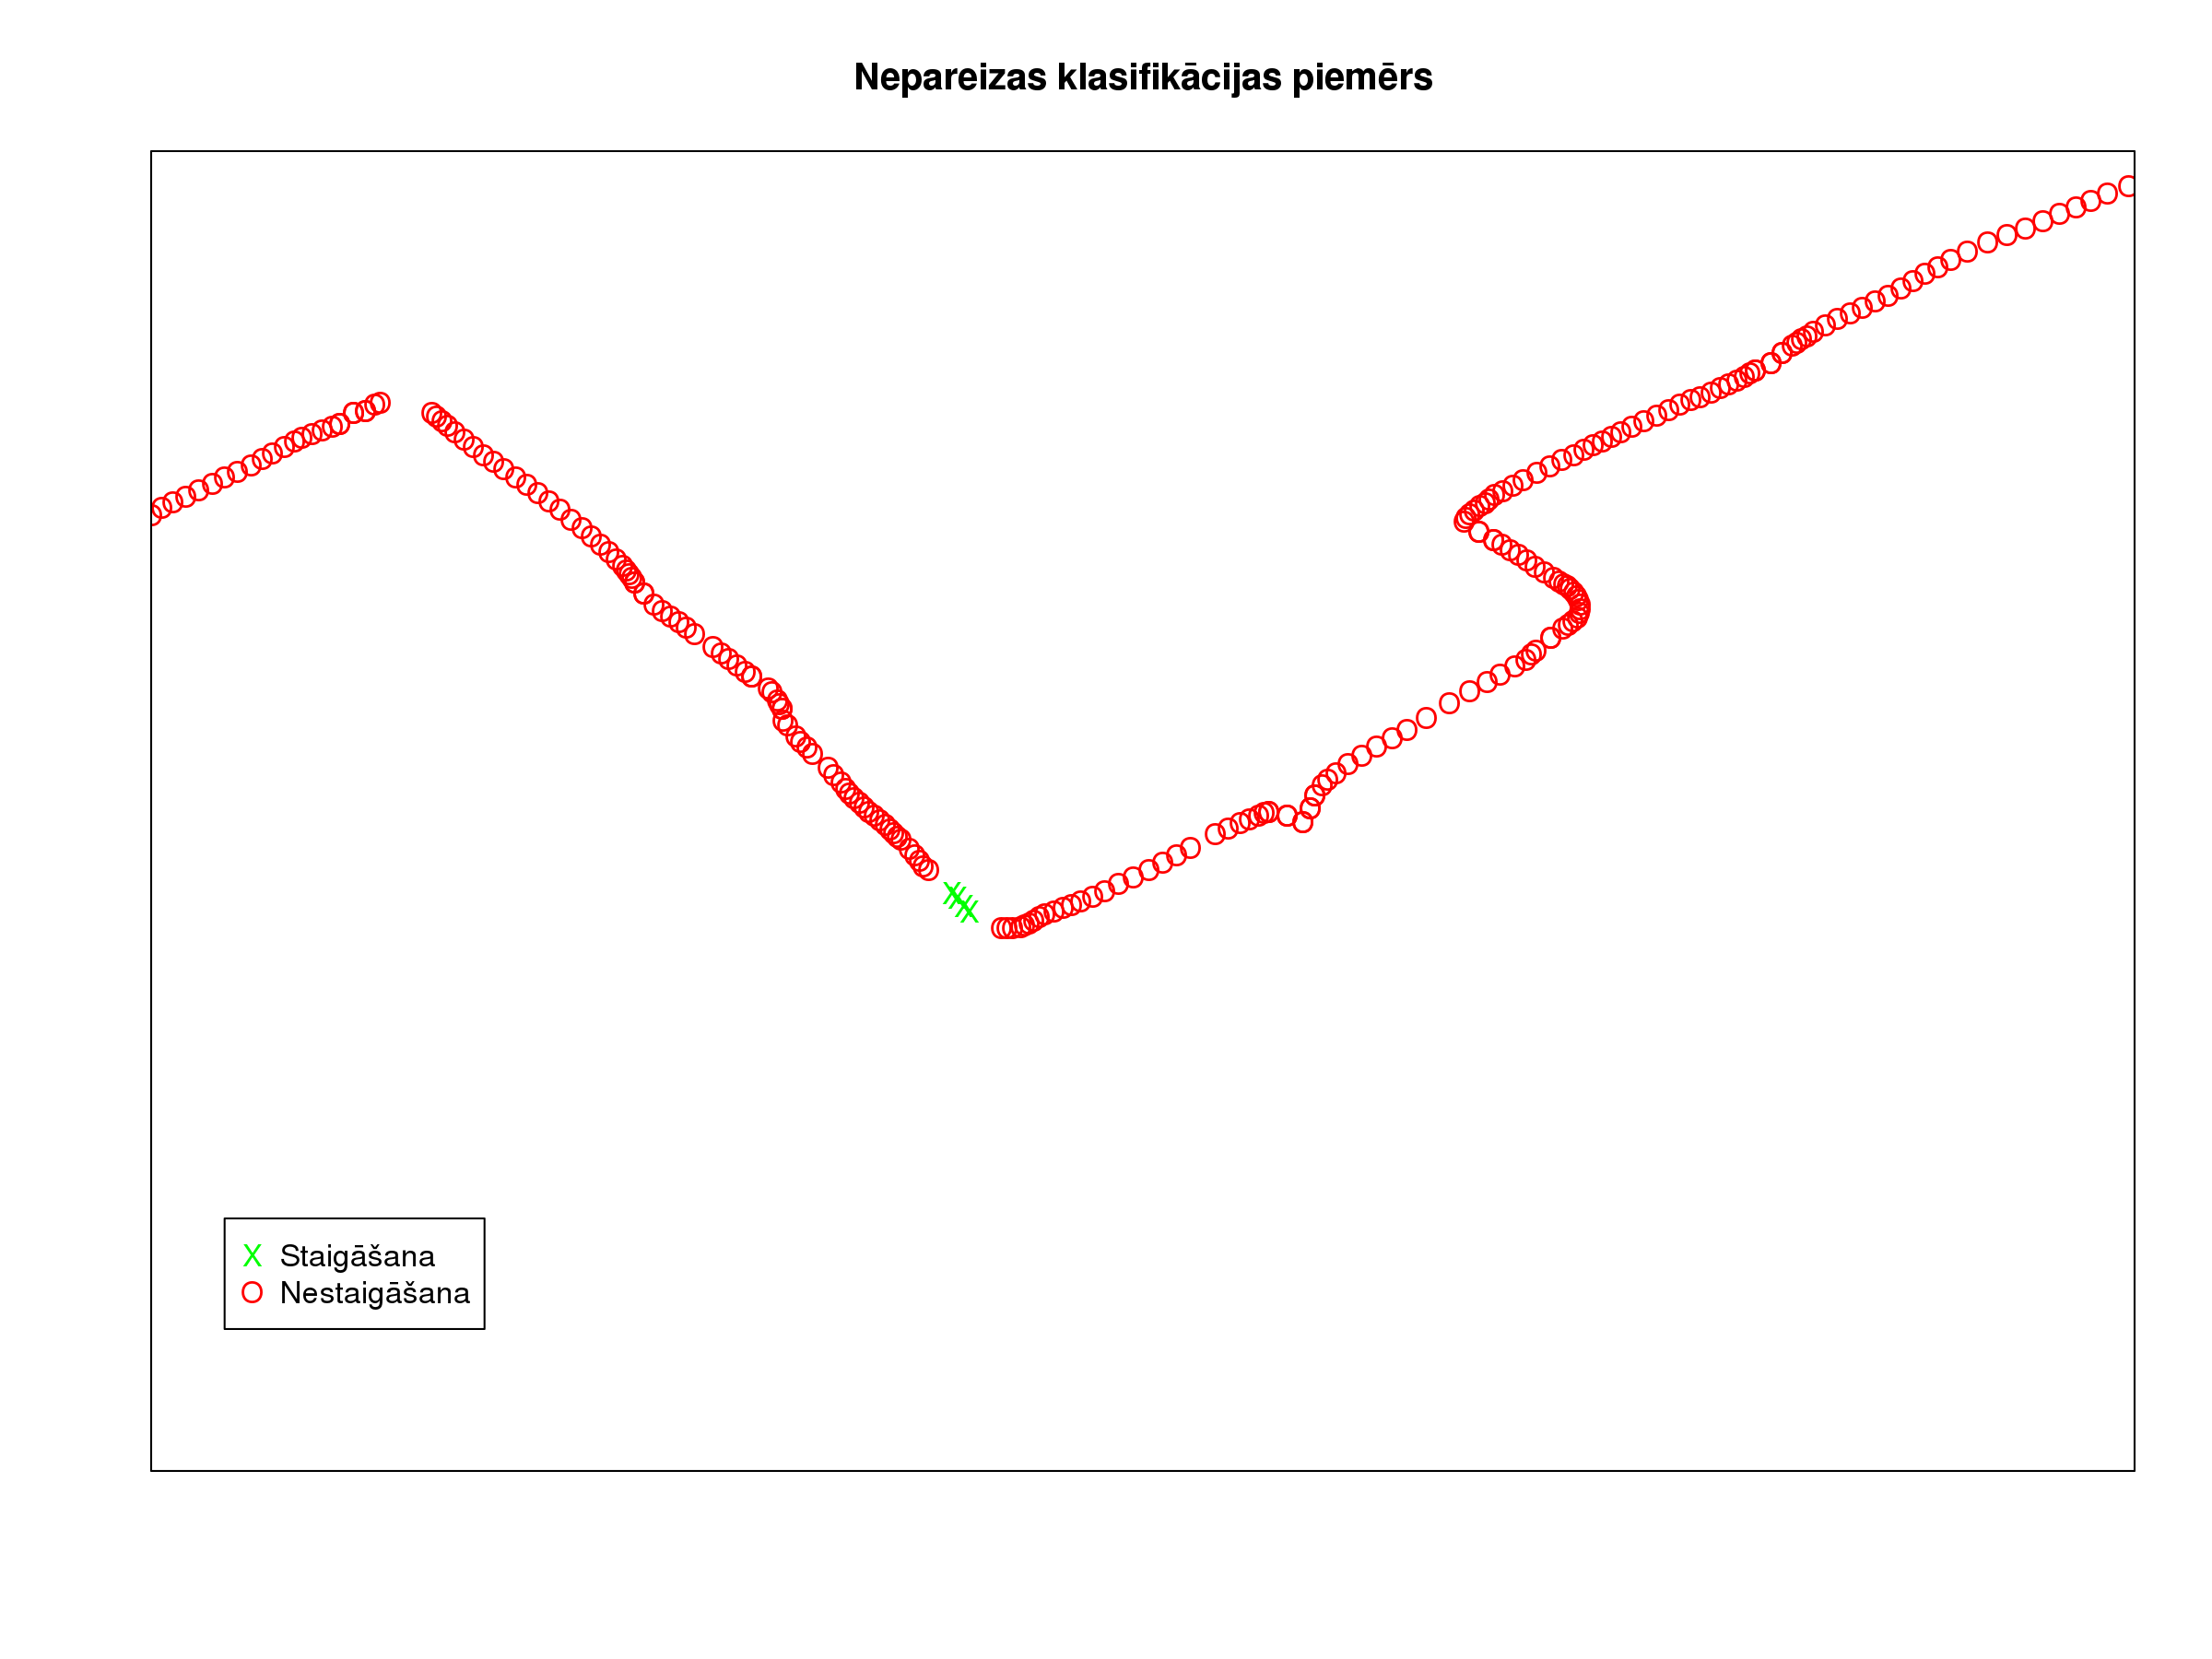
\includegraphics[scale=0.3]{img/wrong_segmentation}
\end{frame}

\begin{frame}
  \frametitle{Kā tās labot?}
  \begin{itemize}
    \item Klasterizācijas kļūdas – ar papildus pazīmēm
    \item Segmentēšanas kļūdas – ieviešot heiristiku
  \end{itemize}
\end{frame}

\begin{frame}
  \frametitle{Kādi ir secinājumi?}
  \begin{itemize}
    \item Augstā frekvencē ierakstītus GPS datus ir iespējams sadalīt segmentos un grupēt
      pēc transporta veida
    \item Paātrinājums ir laba pazīme, pēc kuras šo grupēšanu veikt
    \item Ar paātrinājumu vien nepietiek
  \end{itemize}
\end{frame}

\begin{frame}
  \fontsize{20pt}{0}\selectfont
  \centerline{Paldies par uzmanību!}
  \fontsize{14pt}{0}\selectfont
  \centerline{Jautājumi?}
\end{frame}

\end{document}
